%% Projeto Apostila De Python para pessoas sem conhecimento prévio de porcaria nenhuma
%% mas que querem fazer bonito
%% Parte 2

%% O preâmbulo a seguir coloca o documento todo no formato ABNT puro.
%% Devido a interpretação local (das muitas possíveis) da ABNT, alguns
%% podem questionar o formato.

%% abtex2-modelo-livro.tex, v-1.9.7 
%% Copyright 2012-2018 by abnTeX2 group at http://www.abntex.net.br/
%%
%% This work may be distributed and/or modified under the
%% conditions of the LaTeX Project Public License, either version 1.3
%% of this license or (at your option) any later version.
%% The latest version of this license is in
%%   http://www.latex-project.org/lppl.txt
%% and version 1.3 or later is part of all distributions of LaTeX
%% version 2005/12/01 or later.
%%
%% This work has the LPPL maintenance status `maintained'.
%%
%% Further information is available on 
%% http://www.abntex.net.br/
%% 


\documentclass[
	% -- opções da classe memoir --
%	10pt,				% tamanho da fonte
	12pt,				% tamanho da fonte
	openright,			% capítulos começam em pág ímpar (insere página vazia caso preciso)
	twoside,			% para impressão em recto e verso. Oposto a oneside
	a4paper,			% tamanho do papel. 
	%a5paper,			% tamanho do papel. 
	% -- opções da classe abntex2 --
	%chapter=TITLE,		% títulos de capítulos convertidos em letras maiúsculas
	%section=TITLE,		% títulos de seções convertidos em letras maiúsculas
	%subsection=TITLE,	% títulos de subseções convertidos em letras maiúsculas
	%subsubsection=TITLE,% títulos de subsubseções convertidos em letras maiúsculas
	% -- opções do pacote babel --
	english,			% idioma adicional para hifenização
	french,				% idioma adicional para hifenização
	brazil,				% o último idioma é o principal do documento
	sumario=tradicional
]{abntex2}

% compilação de fontes


\usepackage{mathtools}
\usepackage{amsfonts}
\usepackage{mathrsfs} % para mathscr

\usepackage{ifxetex}
\ifxetex
  % % se for utilizar as fontes do sistema: **escolha sua fonte**
    % comandos de fontes
\usepackage{mathspec}
\setmathsfont(Digits,Latin,Greek){Minion Pro}
\setmathrm{Minion Pro}
\setmainfont[Numbers=OldStyle]{Minion Pro} %fonte principal (serifada)
\setsansfont[Scale=0.9]{Myriad Pro} %fonte sem serifas
\setmonofont[Scale=MatchLowercase]{Consolas} % fonte monoespaçada
  
  \usepackage{polyglossia} %always load polyblossia after fonts for digits in math mode
  \setmainlanguage{brazil}
  \setotherlanguages{french,english,spanish,german,italian}  
  
\else
  % % se for utilizar pdflatex
\usepackage[utf8]{inputenc}
\usepackage{newtxmath} 
\usepackage{Alegreya}
\usepackage{AlegreyaSans}
\usepackage[lf]{FiraMono}
\usepackage[italic]{mathastext}
\fi

%% Observação: o pacote polyglossia pode apresentar erro ao ser utilizado com ifxetex + babel. 
%% Se isso acontecer, atualize o pacote para a versão mais recente ou utilize somente uma das sequências (pdflatex ou xelatex), comentando ou apagando a outra.

\usepackage{microtype} 				% para melhorias de justificação
\usepackage[dvipsnames]{xcolor} 		% para cores
\usepackage{graphicx} 			% para imagens
\usepackage{booktabs,tabularx,rotating}	% para tabelas
\usepackage{mdframed} 				% para caixas de texto como na CIP do verso do título
\usepackage{multicol}				% tabelas com colunas mescladas
\usepackage{lettrine}				% letras capitulares
\usepackage{xspace} 				% para nao precisar de espaços com {} depois de comandos
									% como \LaTeX e abreviações criadas pelo usuário
\usepackage{lipsum} 				% para texto de preenchimento de exemplo
\usepackage{leading}				% espaçamento entrelinhas (leading)
\leading{13pt}

% ---
% Pacotes de citações
% ---
\usepackage[brazilian,hyperpageref]{backref}	 % Paginas com as citações na bibl
\usepackage[alf]{abntex2cite}	% Citações padrão ABNT

% ---
% Configurações do pacote backref
% Usado sem a opção hyperpageref de backref
\renewcommand{\backrefpagesname}{Citado na(s) página(s):~}
% Texto padrão antes do número das páginas
\renewcommand{\backref}{}
% Define os textos da citação
\renewcommand*{\backrefalt}[4]{
	\ifcase #1 %
		Nenhuma citação no texto.%
	\or
		Citado na página #2.%
	\else
		Citado #1 vezes nas páginas #2.%
	\fi}%
% ---

% ---
% Informações do documento
% ---
\titulo{Apostila de Python Para Iniciantes Parte 2}
\autor{Engenheiros que dizem: ``Nih!'' \\ 
         Giovani Zanelatto, Victor Bergossi, Gabriel Selow, Leo, 41 9687-1698, 41 9846-7571
}
\data{2020, v-0.0.0}
\preambulo{Breve sinopse da Apostila}
\local{Curitiba}
\instituicao{UTFPR}

% alterando o aspecto da cor azul
\definecolor{blue}{RGB}{41,5,195}

% informações do PDF
\makeatletter
\hypersetup{
     	%pagebackref=true,
		pdftitle={\@title}, 
		pdfauthor={\@author},
    	pdfsubject={\imprimirpreambulo},
	    pdfcreator={LaTeX with abnTeX2},
		pdfkeywords={abnt}{latex}{abntex}{abntex2}{livro}, 
		colorlinks=true,       		% false: boxed links; true: colored links
    	linkcolor=blue,          	% color of internal links
    	citecolor=blue,        		% color of links to bibliography
    	filecolor=magenta,      		% color of file links
		urlcolor=blue,
		bookmarksdepth=4
}
\makeatother
% ---


% ---
% Estilo de capítulos
%
% \chapterstyle{pedersen} 
% \chapterstyle{lyhne} 
%\chapterstyle{madsen} 
\chapterstyle{veelo} 
%
% Veja outros estilos em:
% https://www.ctan.org/tex-archive/info/MemoirChapStyles
% ---

% para cabeçalhos sem estar em maiúsculas
%\nouppercaseheads 

% -----
% Declarações de cabecalhos 
% -----
% Cabecalho padrao
\makepagestyle{abntbookheadings}
\makeevenhead{abntbookheadings}{\ABNTEXfontereduzida\thepage}{}{\ABNTEXfontereduzida\textit\leftmark}
\makeoddhead{abntbookheadings}{\ABNTEXfontereduzida\textit\rightmark}{}{\ABNTEXfontereduzida\thepage}
\makeheadrule{abntbookheadings}{\textwidth}{\normalrulethickness}

% Cabecalho do inicio do capitulo
\makepagestyle{abntbookchapfirst}
\makeoddhead{abntbookchapfirst}{}{}{}

% Configura layout para elementos textuais
\renewcommand{\textual}{%
  \pagestyle{abntbookheadings}%
  \aliaspagestyle{chapter}{abntbookchapfirst}% customizing chapter pagestyle
  \nouppercaseheads%
  \bookmarksetup{startatroot}% 
}
% ---



% Margens do documento 
%% (margens do abntex2 não combinam nem com A5 nem com estilos de capítulo da
% classe memoir.)
\setlrmarginsandblock{2.5cm}{3.5cm}{*}
\setulmarginsandblock{2.5cm}{3.5cm}{*}
\checkandfixthelayout
% ---


%% para inserção de trechos de código Python
\usepackage{pythonhighlight}
\usepackage[T1]{fontenc}
% ---
% Início do documento
% ---
\begin{document}
\frenchspacing

\frontmatter

% ---
% Capa principal
% ---
\begin{titlingpage}
\phantom{xxx}
\vspace{0.5cm}
\huge
\raggedright
\imprimirautor\\
\vspace{2.5cm}
\huge 
{\raggedleft
%\scalebox{-1}[1]{
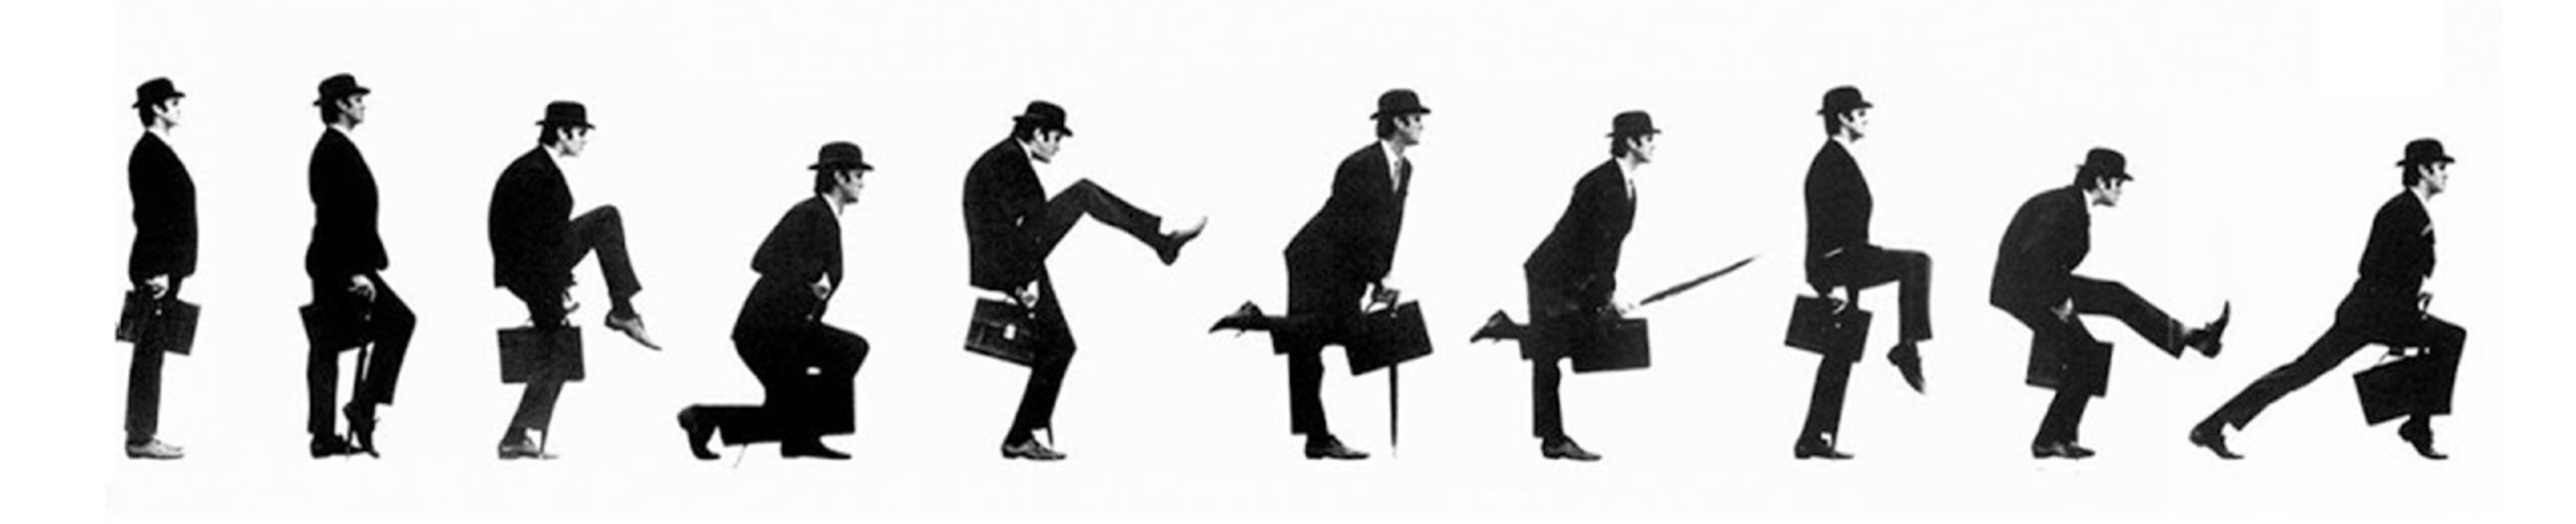
\includegraphics[scale=0.3]{MontyPythonSillyWalkDiagram.pdf}\\[1cm]
%}
%%\includegraphics[scale=0.9]{abntex2-modelo-img-marca.pdf}\\[1cm]
\textit{\textcolor{blue}{\imprimirtitulo}}\\[1cm]
}
\centering 
% %este é um símbolo que só aparecerá com a fonte Minion.
\vfill
\Large
% %este é um símbolo que só aparecerá com a fonte Minion.
\imprimirinstituicao
\end{titlingpage}
% ---

% ---
% Contra-capa
% ---
\begin{titlingpage}

\phantom{xxx}
\vspace{0.5cm}
\huge
\raggedright
\imprimirautor\\
\vspace{2.5cm}
\huge 
{\raggedleft
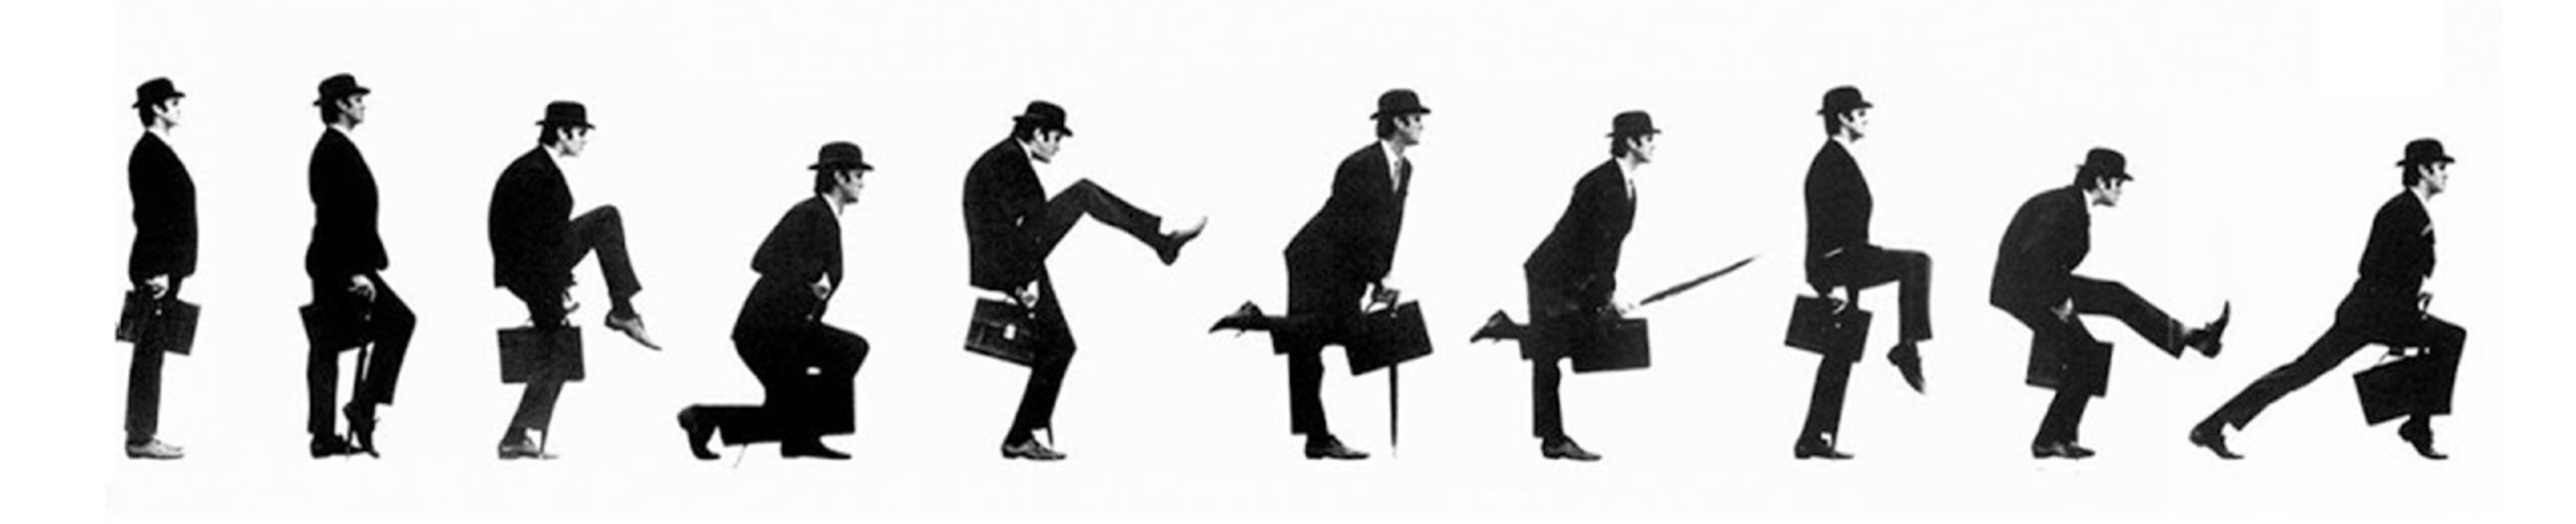
\includegraphics[scale=0.3]{MontyPythonSillyWalkDiagram.pdf}\\[1cm]
%%\includegraphics[scale=0.9]{abntex2-modelo-img-marca.pdf}\\[1cm]
\textit{\textcolor{blue}{\imprimirtitulo}}\\[1cm]
}
\centering 
% %este é um símbolo que só aparecerá com a fonte Minion.
\vfill
\Large
% %este é um símbolo que só aparecerá com a fonte Minion.
\imprimirinstituicao
% ---

% ---
% Verso da contra-capa
% ---
\clearpage
\ABNTEXfontereduzida
%\raggedright
© 2020 \imprimirautor \space \& \imprimirinstituicao
%este é só um exemplo de copyright.

Qualquer parte desta publicação pode ser reproduzida, desde que citada a fonte.

\vspace*{\fill}

\begin{center}
Dados Internacionais de Catalogação na Publicação (\textsc{cip})
Câmara Brasileira do Livro, \textsc{sp}, Brasil
\end{center}

\begin{mdframed}
\noindent Zanelatto, Giovani. %% autor como referenciado em citações;

\imprimirtitulo. / \imprimirautor. -- \imprimirlocal: \imprimirinstituicao\ 
 2020.

\medskip

Bibliografia.

ISBN XXXX-XXXX-XX.

\medskip

1. Programas de computador. 2. Python. 3. Fundamentos. 4. Receitas.

\end{mdframed}

\end{titlingpage}
% ---

% ---
% inserir lista de ilustrações
% ---
\pdfbookmark[0]{\listfigurename}{lof}
\listoffigures*
\cleardoublepage

% ---
% inserir lista de tabelas
% ---
\pdfbookmark[0]{\listtablename}{lot}
\listoftables*
\cleardoublepage
% ---

% ---
% inserir o sumario
% ---
\pdfbookmark[0]{\contentsname}{toc}
\tableofcontents*
\cleardoublepage
% ---

% ------------------------------------------------------------
% Início da parte textual
% ------------------------------------------------------------
%\textual
\mainmatter
% ------------------------------------------------------------
\OnehalfSpacing
% ------------------------------------------------------------
\chapter*[Introdução]{Introdução} %% título do capitulo
\addcontentsline{toc}{chapter}{Introdução}  %% comando para colocar o título do capítulo no table of contents
% ------------------------------------------------------------

\lettrine[nindent=0.35em,lhang=0.40,loversize=0.3]{A}{ssuminos} que o leitor desta apostila
já leu a primeira parte desta apostila e tem domínio sobre a sintaxe básica de Python. Esta apostila contém a parte de aplicações práticas e deve ser encarada como um livro de receitas. Assim como um livro de receitas culinárias, o que está escrito aqui não cobre todo o espectro de problemas e soluções. Também não são receitas absolutas e cabe ao leitor experimentá-las e modificá-las ao seu gosto ou necessidade.

Para tanto é fundamental que as receitas sejam compreendidas, e para isso é de extrema importância que o leitor não se limite a ler, mas pratique com atenção o exemplo e se esmere no exercício proposto. Assim como na cozinha é a prática diária que aprimora o ``Chef'' de sucesso.


\section[Uma breve amostra] {Uma breve amostra}%\addcontentsline{toc}{section}{Uma breve amostra}
Mesmo assumindo uma leitura prévia apresentamos uma revisão fundamental no capítulo \ref{RevisaoPython}.
Faremos uma breve introdução de estatística e introduziremos o NumPy e o MatPlotLib no capítulo \ref{EstatisticaPython}





% ------------------------------------------------------------
\chapter{Revisão Python}\label{RevisaoPython}
% ------------------------------------------------------------
Revisão dos conceitos básicos
Jupyter Notebook




% ------------------------------------------------------------
\chapter{Estatística básica e numpy/matplotlib}\label{EstatisticaPython}
% ------------------------------------------------------------
%Conceitos básicos de estatística (Média, mediana, moda, desvio padrão e variância)
%Operações com array usando a biblioteca numpy e arrays padrões 
%\cite{NumPyUserGuideRelease1.18.1}
%% ------------------------------------------------------------
%\chapter{Estatística básica e numpy/matplotlib}\label{EstatisticaPython}
%% ------------------------------------------------------------
%Conceitos básicos de estatística (Média, mediana, moda, desvio padrão e variância)
%Operações com array usando a biblioteca numpy e arrays padrões 

\section{NumPy}
Escrever sobre o NumPy...
O NumPy é a abreviação de Numerical Python e é uma biblioteca Python escrita para trabalhar com vetores e matrizes, incluindo funções na área de álgebra linear e transformadas de Fourier. \cite{NumPyUserGuideRelease1.18.1}



\section{Resumo de estatísitca}

Em geral, estatísticos não gostam de serem denominados de matemáticos. A Estatística é tratada por seus especialistas (estatísticos) como uma ciência à parte da Matemática. Assim como a Física ou a Engenharia, a Estatística utiliza a Matemática como ferramenta. Abordaremos neste breve resumo apenas as definições básicas e fundamentais, sem entrar em mais detalhes. Se seu problema envolver algo mais elaborado ou se você tiver curiosidade sobre este fascinante tema, recomendamos a leitura das referências:   \cite{Est_Bussab}, \cite{Est_NilzaNunes}, \cite{EST_Montgomery} e \cite{Est_Meyer}.


\subsection{Definições Importantes}
Para a situação de dados discretos:
\subsubsection{Média Aritmética}
Dado um conjunto de $12$ valores: $93$, $94$, $95$, $97$, $98$, $98$, $100$, $101$, $101$, $104$, $105$, e $108$ a média aritmética $\bar x$ é dada por:
\[
\bar x = \frac{93+94+95+97+98+98+100+101+101+104+105+108}{12}  = 99,5   
\]
Em uma notação mais compacta e elegante escrevemos que a média aritmética de um conjunto de $N$ valores $x_1$ até $x_N$ é dado por
\[
    \bar x = \frac{1}{N}\sum_{i=1}^N x_i = \frac{2}{N} (x_1 + x_2 + x_3 + \cdots + x_N )
\]

%\usepackage{pythonhighlight} %% google ctan
Definindo uma função em Python:
%%% verificar este trecho de código!%%%%%%%%%%%%
\begin{python}
    def media_aritm(x):
    if len(x) == 0:
        return 0
    else:
        soma = 0
        for i in x:
            soma = soma + i
        return soma/len(x)
\end{python}

Alternativamente podemos usar a função sum() e Escrever
\begin{python}
    def media_aritm(x):
         return sum(x)/len(x)
\end{python}

Utilizando a biblioteca NumPy simpesmente invocamos o método:
\begin{python}
    numpy.mean(x)
\end{python}





% ------------------------------------------------------------
\chapter{Matplotlib}
% ------------------------------------------------------------

Visualização de dados com matplotlib



% ------------------------------------------------------------
\chapter{PANDAS}
% ------------------------------------------------------------

Operações com DataFrames, planilhas e arquivos de dados com Pandas

% ------------------------------------------------------------
\chapter{PANDAS / SEABORN / PLOTLY}
% ------------------------------------------------------------

Visualização de dados com seaborn, plotly e pandas

% ------------------------------------------------------------
\chapter{SCIKIT-LEARN / STATSMODEL - I}
% ------------------------------------------------------------

Conceitos matemáticos dos conteúdos trabalhados no capítulo
Regressão Linear
Regressão Linear Multipla

% ------------------------------------------------------------
\chapter{SCIKIT-LEARN / STATSMODEL - II}
% ------------------------------------------------------------

Conceitos matemáticos dos conteúdos trabalhados no capítulo
Regressão Logística
ANOVA

% ------------------------------------------------------------
\chapter{SCIKIT-LEARN/STATSMODEL - III}
% ------------------------------------------------------------

Conceitos matemáticos dos conteúdos trabalhados no capítulo
KNN (K Nearest Neighbors) 
SVM (support vector machines)




% ------------------------------------------------------------
\postextual % pós-textual
% ------------------------------------------------------------

% ------------------------------------------------------------
\bibliography{Apostila_Python_References}
\end{document} %% documento termina aqui






% ------------------------------------------------------------
\chapter{Exemplos de imagens}
% ------------------------------------------------------------

\lipsum[1]

\begin{figure}
\centering
\includegraphics[width=0.6\linewidth]{example-image-a}
\caption{Exemplo de imagem.}
\label{fig:exemplo}
\end{figure}

\lipsum[6]





\lipsum[7]

% ------------------------------------------------------------
\chapter{Exemplos de tabela}
% ------------------------------------------------------------

\section{Uma seção}

\lipsum[8]

\begin{table}
\caption{Pequeno vocabulário de design de livros\label{vocabulario-texto}}
\ABNTEXfontereduzida
\begin{tabular}{p{4cm}p{4cm}}
\toprule
\textit{Termo em inglês} & \textit{Termo em português}\\
\midrule
\ABNTEXfontereduzida
title page & folha de rosto.\\

cover & capa\\

back cover & quarta capa ou contra-capa ou verso da capa\\

bastard title ou half title & falsa folha de rosto. Tem só o título do livro.\\

table of contents & sumário\\

text block ou book block & miolo\\

print space (alemão: \textit{Satzspiegel}) & mancha gráfica\\

section, gathering, quire (especialmente se não impresso), signature & caderno\\

leaf = folio (latim) & folha, composta de recto (lat.) (anverso/frente) e verso (lat.) (verso). Geralmente o recto é página ímpar, e verso é página par.\\

hardcover & capa dura.\\

endpaper/endsheet & folha de guarda. Folha de papel para prender o miolo do livro na capa dura.\\

dust jacket, dust cover, book jacket, dust wrapper & sobrecapa. Geralmente de papel, para cobrir capas duras.\\

front matter & parte pré-textual.\\

main matter & parte textual\\

back matter & parte pós-textual. Composta por epílogo, posfácio, apêndice, glossário, bibliografia, índice remissivo (inglês: index), colofão etc.\\

colophon & colofão. Breve descrição sobre aspectos da publicação do livro. \\

running headers & títulos correntes\\

volume & volume. Conjunto de páginas encadernadas.\\

\bottomrule
\end{tabular}
\footnotesize Fontes:\\
\url{http://pt.wikipedia.org/wiki/Design_de_livros}\\
\url{http://en.wikipedia.org/wiki/Book_design}\\
\url{http://static.lexicool.com/dictionary/RX7KW614433.pdf}\\
\end{table}


\begin{table}
\caption{Exemplo de tabela utilizando o pacote \textsf{booktabs}.}
\centering
\begin{tabular}{llr}
\toprule
\multicolumn{2}{c}{Item} \\
\cmidrule(r){1-2}
Animal    & Description & Price (\$) \\
\midrule
Gnat      & per gram    & 13.65      \\
          & each        & 0.01       \\
Gnu       & stuffed     & 92.50      \\
Emu       & stuffed     & 33.33      \\
Armadillo & frozen      & 8.99       \\
\bottomrule
\multicolumn{3}{l}{\ABNTEXfontereduzida Fonte: \url{http://en.wikibooks.org/wiki/LaTeX/Tables}}
\end{tabular}
\end{table}

\lipsum[9]

% ------------------------------------------------------------
\postextual % pós-textual
% ------------------------------------------------------------

% ------------------------------------------------------------
\bibliography{Apostila_Python_References}
%\bibliography{abntex2-modelo-references} % insere o arquivo de bibliografia
% ------------------------------------------------------------

% ------------------------------------------------------------
% Colofão: última página com informações sobre a composição do livro.
\cleardoublepage
\thispagestyle{empty} 

Sinta-se convidado a participar do projeto \abnTeX! Acesse o site do projeto em
\url{http://www.abntex.net.br/}. Também fique livre para conhecer, estudar,
alterar e redistribuir o trabalho do ABN\TeX, desde que os arquivos modificados
tenham seus nomes alterados e que os créditos sejam dados aos autores originais,
nos termos da ``The \LaTeX\ Project Public
License''\footnote{\url{http://www.latex-project.org/lppl.txt}}.

Encorajamos que sejam realizadas customizações específicas deste documento.
Porém, recomendamos que ao invés de se alterar diretamente os arquivos do
\abnTeX, distribua-se arquivos com as respectivas customizações.
Isso permite que futuras versões do \abnTeX~não se tornem automaticamente
incompatíveis com as customizações promovidas. Consulte
\citeonline{abntex2-wiki-como-customizar} para mais informações.

\end{document}
